\documentclass[runningheads,a4paper]{llncs}
\usepackage{cite}
\usepackage{amssymb}
\usepackage{graphicx}
\usepackage{eurosym}

\usepackage{pgfplots}
\usepackage{subfig}
\usepackage[hidelinks]{hyperref}
\def\UrlBreaks{\do\/\do-}
\usepackage{url}
\usetikzlibrary{arrows,calc}
\pgfplotsset{width=3.4cm,compat=1.7}
\renewcommand{\UrlFont}{\footnotesize}
\usepackage{listings, color}


\authorrunning{Ran Wei, Timothy P. Kelly, Richard Hawkins}

\makeatletter
\renewcommand\subsubsection{\@startsection{subsubsection}{3}{\z@}%
	{-18\p@ \@plus -4\p@ \@minus -4\p@}%
	{4\p@ \@plus 2\p@ \@minus 2\p@}%
	{\normalfont\normalsize\bfseries\boldmath
		\rightskip=\z@ \@plus 8em\pretolerance=10000 }}
\renewcommand\paragraph{\@startsection{paragraph}{4}{\z@}%
	{-12\p@ \@plus -4\p@ \@minus -4\p@}%
	{2\p@ \@plus 1\p@ \@minus 1\p@}%
	{\normalfont\normalsize\itshape
		\rightskip=\z@ \@plus 8em\pretolerance=10000 }}
\makeatother




\begin{document}
 
\title{\textbf{DEIS: Dependability Engineering Innovation for Cyber Physical Systems}}
\author{Ran Wei\and Timothy P. Kelly \and Richard Hawkins}
\institute{Department of Computer Science, \\ University of York, United Kingdom \\ ran.wei, tim.kelly, richard.hawkins@york.ac.uk}
\maketitle


\begin{abstract}
The open and cooperative nature of Cyber-Physical Systems (CPS) poses a significant new challenge in assuring dependability. The DEIS project addresses this important and unsolved challenge by developing technologies that enable a science of dependable system integration. 
Such technologies facilitate the efficient synthesis of components and systems based on their dependability information, covering application domains such as automotive, railways, home automation and healthcare.

The DEIS project will bring significant impact to the CPS market by providing new engineering methods and tools reducing development time and cost of ownership, as well as supporting integration and interoperability of dependability information over the product life-cycle and over the supply chain.
\end{abstract}


\section{Project Information}
\begin{itemize}
	\item \textbf{Project acronym}: DEIS
	\item \textbf{Project title}: Dependability Engineering Innovation for Cyber Physical Systems (CPS)
	\item \textbf{Project funding}: Total cost \euro 4,889,290 (funded by H2020-EU.2.1.1)
	\item \textbf{Project partners}: AVL List GmbH (project coordinator), Siemens AG, General Motors Powertrain-Europe SRL, Ideas \& Motion SRL, Portable Medical Technology Ltd, Fraunhofer Gesellschaft zur F{\"o}rderung der angewandten forschung E.V, University of Hull, University of York, Politecnico of Milano, RSRC at Dundalk Institute of Technology.
	\item \textbf{Project start date/duration}: 30 January, 2017 (36 months).
\end{itemize}

\section{Introduction}
It is expected that in the future, the physical and digital worlds will merge into a largely connected globe. This is backed by the emergence of notions such as Cyber-Physical-Systems (CPS). 
%At the moment, CPS technologies have been applied in a broad range fo domains, including smart grids, smart homes, smart health, intelligent transportation, etc. 
CPS harbour the potential for vast economic and societal impact in domains such as automotive, health care and home automation. At the same time, if these systems fail, they may cause harm and lead to temporary collapse of important infrastructures, with catastrophic consequences for industry and society. 
Therefore, in order to realise the full potential for innovation of CPS, it is important to ensure the dependability of CPS.
% - especially in relation to security and safety, as security and safety are important aspects in CPS, breaches to any of them can cause catastrophic events.

CPS are typically loosely connected and come together as temporary configurations of smaller systems which dissolve and give place to other configurations. Therefore, the configurations a CPS may assume over its lifetime are unknown and potentially infinite. Thus, currently available approaches are not possible to assure the dependability of CPS and it is a grand technology challenge to address the dependability of CPS. 

The DEIS project identifies this challenge and takes a first step towards dependability assurance of CPS by focusing on system safety and security, since assuring safety of such systems is an indispensable prerequisite in order to realise the economic and social potential of CPS.






\section{Identified Challenges and Project Concept}
A DDI is potentially a very useful digital artefact - It is a versatile dependability assurance case, the utility of which spans from component design to in-the-field operation of a CPS. However, the production and use of DDIs for heterogeneous systems poses a number of significant technological and engineering challenges that are pertinent and important in industry and motivate the objectives of the DEIS project. 

DEIS identifies the following challenges for DDI:
\clearpage
\begin{enumerate}
	\item \textbf{Universal exchange of dependability information}
		\begin{itemize}
			\item Currently there is a lack of common model representations for the exchange of dependability information. Thus, a precondition for DDI is the existence of an open dependability metamodel. 
			\item DDIs should be sufficiently expressive to enable the component integrator to compile DDIs from the sub-components DDIs, for system synthesis.
			\item DDIs should optionally shield sensitive details through abstraction to protect the component provider's intellectual property. 
		\end{itemize}
	\item \textbf{Efficient dependability assurance across industries and value chains}
		\begin{itemize}
			\item Component providers should be able to generate DDIs based on the dependability information of their components/systems that is already available in their existing tools.
			\item It must be possible to include the information contained in DDIs into the dependability assurance lifecycle and tool chain of the component integrator, to cater with the change in component/system requirements and integration context.
			\item Dependability should be considered from the early stages of design, so that a model-based approach can be adopted to enable automation, and eventually the automatic synthesis of systems/DDIs.
		\end{itemize}
	\item \textbf{Dependable integration of systems in the field}
		\begin{itemize}
			\item In CPS, dependability cannot be fully assured prior to deployment. This requires certain degree of automation in evaluation of DDIs. Thus, DDIs must become executable specifications.
			\item DDIs must be stored in a centralised repository so that they can be accessed in a uniform way, and changes in them are synchronised.
			\item Fully automated evaluation of DDIs required for highly dynamic environments.
		\end{itemize}
\end{enumerate}

\begin{figure}[ht!]
	\centering
	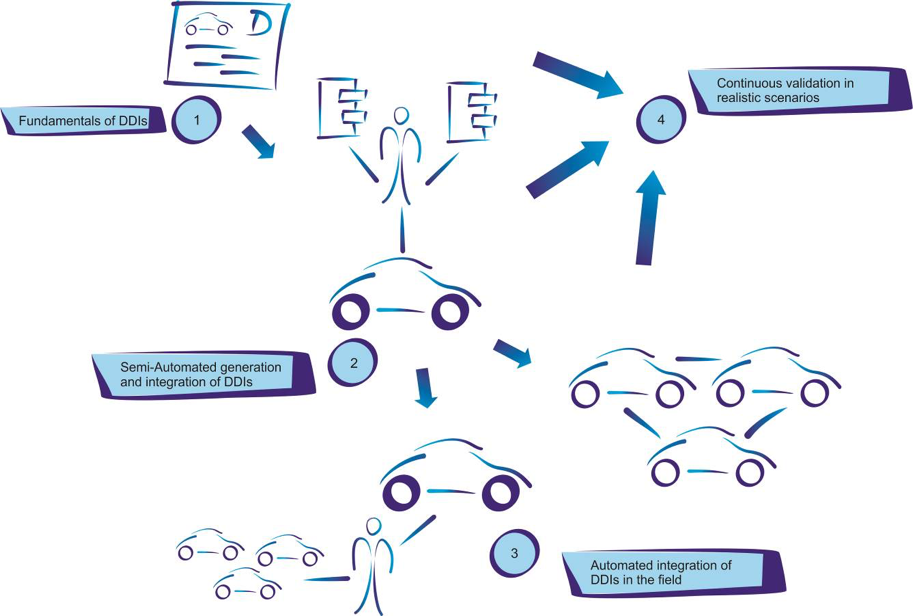
\includegraphics[width=1\linewidth]{./fig/proj_concept.png}
	\caption{DEIS project concept}
	\label{fig:proj_concept}
\end{figure}

To address these major technology and research challenges, the DEIS project sets out a four-stage innovation cycle, as illustrated in Figure \ref{fig:proj_concept}. The first stage aims at the fundamentals of DDIs, such as the definition of a universal format of DDIs based on an open information model for the exchange of dependability information. The second stage is to provide semi-automated and increasingly automated support for generating DDIs out of existing design and safety models, as well as for integrating the DDIs of sub-components into DDIs of larger systems by integrators. The third stage facilitates dependable integration of systems in the field though automated evaluation of DDIs that includes the concept of executable DDIs on-board. Finally, the fourth stage is to have continuous validation of the project results in realistic scenarios and case studies.





\section{Project Objectives}
\label{section4}
Based on the identified challenges and the concept, the objectives of the DEIS project are set out as the following.

%\subsection{Objective 1. An open dependability exchange (ODE) metamodel and a universal format for specifying DDIs}
\subsubsection{Objective 1. An open dependability exchange (ODE) metamodel and a universal format for specifying DDIs} 
Based on existing work, DEIS will produce an Open Dependability Exchange (ODE) metamodel. ODE provides the means to express, connect and communicate dependability information.  
With ODE, it would be possible to specify the level of trust of assured dependability properties with respect to the trust of the issuer and to the trust level of the promised services during field operation. DDIs should also be generated based on the information defined in ODE. 
%Where ODE may contain detailed intellectual property, DDIs will be defined at a more abstract level. 
DDIs will also be formalised in order to support their semi-automated evaluation.

Measurable sub-objectives of objective 1 are:
\begin{enumerate}
	\item Definition of the Open Dependability Exchange (ODE) metamodel
	\item Definition of general form of Digital Dependability Identity (DDI)
	\item Tooling support for the manual modelling of DDIs
	\item Tooling support to check the validity of DDIs
\end{enumerate}

\subsubsection{Objective 2. A framework for the creation and modular synthesis of DDIs}
Once an appropriate format for the ODE and DDIs is defined, DEIS will provide support for the creation and modular synthesis of DDIs from existing dependability information. Such support is a prerequisite for the practical applicability of the approach. Thus a framework that serves such purpose will be developed, covering the following sub-objectives:

\begin{enumerate}
	\item Tooling support for expressing existing dependability models in ODE-compliant format
	\item Algorithms and tooling support for synthesis of DDIs
	\item Algorithms and tooling support for integration of DDIs into the dependability assurance cases
	\item Algorithms and tooling support for change-impact analysis on DDIs
\end{enumerate}

\subsubsection{Objective 3. A framework for the in-the-field dependability assurance in CPS}
A framework which enables the dependable integration of open CPS is required. Such framework consists a centralised DDI registry which is publicly available on-the-cloud. By using the centralised DDI registry, system manufacturers can check if their systems can be dependably integrated with already existing systems. Beside the centralised DDI registry, the framework should also enable on-board evaluation. With on-board evaluation, systems carry DDIs with them and evaluate if they can collaborate with each other in the field.

The framework covers the following sub-objectives:

\begin{enumerate}
	\item Development of infrastructures for evaluation of integration of new systems in the field
	\item Development of algorithms for the on-board evaluation of DDIs
\end{enumerate}

\subsubsection{Objective 4. Development of autonomous and connected CPS use cases for different application domains, and validation of applicability and scalability of the DDIs}
The scope of the project and the technology it develops is wide reaching and fundamental for CPS and the industries involved in the project (road transport, railway, healthcare). As such, the project results are expected to create significant impact. For this reason, it is a further objective of the project to validate the results in four realistic scenarios based on representative projects. %The first two scenarios are directly related to new systems that can achieve radical cost reduction for automated driving systems, maintaining and improving dependability via DDIs. A further validation will take place in a railway scenario in context of the European Train Control System (ETCS) with the primary goal being to evaluate the applicability of the results across different application domains. The fourth use case is targeting the medical domain with management of patient-related information for clinical decision support.

The studies of the four scenarios covers the following sub-objectives:

\begin{enumerate}
	\item Evaluation of effectiveness of approach
	\item Evaluation of applicability across industries
	\item Evaluation of runtime mechanisms
	\item Evaluation of systems produced in four case studies
\end{enumerate}

\section{Related Work}
In order to ensure successful project results, the project will not aim at developing an entirely new solution. In fact, the project will use, wherever appropriate, the results from other previous and current projects. In particular, projects that are related to DEIS are: 
\begin{itemize}
	\item VETESS: Verification and Testing to Support Functional Safety Standards
	\item SPES XT: Software Platform Embedded Systems
	\item SAFECER: Safety Certification of Software-Intensive Systems with Reusable Components
	\item CESAR: Cost Effective Small AiRcraft
	\item CRYSTAL: CRitical sYStem engineering AcceLeration
	\item SAFE: Safe Automotive soFtware architEcture
	\item EMC$^2$: Embedded Multi-Core systems for Mixed Criticality applications in dynamic and changeable real-time environments
	\item SafeAdapt: Safe Adaptive Software for Fully Electric Vehicles
	\item OPENCOSS: Open Platform for EvolutioNary Certification Of Safety-critical Systems 
	\item D-MILS: Distributed MILS for dependable information and communication infrastructures
	\item MAENAD: Model-based Analysis \& Engineering of Novel Architectures for Dependable electric vehicles
	\item ATESST2: Advancing Traffic Efficiency and Safety through Software Technology phase 2
	\item COMPASS: Comprehensive Modelling for Advanced Systems of Systems
\end{itemize}

The research in DEIS can also be based upon different existing approaches, like Component Fault Trees \cite{Kaiser2003} and HiP- HOPS \cite{Papadopoulos1999} for dependability analysis, GSN \cite{kelly2004goal} for specifying safety cases, SACM \cite{sacm2} for specifying structured assurance cases,  or ConSerts \cite{Schneider2003} as a starting point for runtime certification. All of these approaches were defined by partners involved in DEIS and have proven their value in many practical applications. The fundamental competence and previous work results provided by the partners involved in DEIS therefore build a sound basis, which gives confidence that the project objectives are achievable within the proposed time and budget of the project.

\section{Ambition and Impact}


\vspace{0.2cm}
\noindent\textbf{Acknowledgements} .

\bibliographystyle{unsrt} 
\bibliography{bibliography}  

\end{document}
